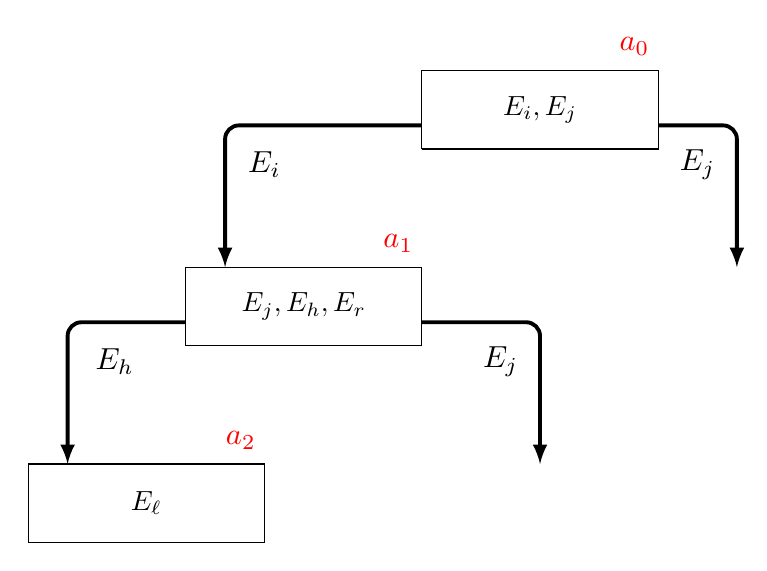
\begin{tikzpicture}

% BLOCS %%%%%%%%%%%%%%%%%%%%%%%%%%%%%%%%%%%%%%%%%%%%%%%%%%%%%%%%%%%%%%%%%%

\draw [color = black, fill = white] (6.0,10.0) -- (6.0,11.0) -- (9.0,11.0) -- (9.0,10.0) --  (6.0,10.0);
\draw [color = black, fill = white] (3.0,7.5) -- (3.0,8.5) -- (6.0,8.5) -- (6.0,7.5) -- (3.0,7.5);
\draw [color = black, fill = white] (1.0,5.0) -- (1.0,6.0) -- (4.0,6.0) -- (4.0,5.0) -- (1.0,5.0);
%\draw [dashed, color = blue, fill = white!92!blue] (4.7,5.3) -- (10.6,5.3) -- (10.6,4.1) -- (8.5,4.1) -- (8.5,3.2) -- (4.7,3.2) -- (4.7,5.3);
% CUBES

\node (P1) at (7.5,10.5) {$\set{E_i,E_j}$};
\node (P2) at (4.5,8.0) {$\set{E_j,E_h,E_r}$};
\node (P3) at (2.5,5.5) {$\set{E_{\ell}}$};


% ETIQUETTES


%\node[scale=1.1, color = blue] at (12.0,10.0) {Depth $0$};
%\node[scale=1.1, color = blue] at (12.0,7.5) {Depth $1$};
%\node[scale=1.1, color = blue] at (12.0,5.0) {Depth $2$};

\node[scale=1.1, color = red] at (8.7,11.3) {$a_0$};
\node[scale=1.1, color = red] at (5.7,8.8) {$a_1$};
\node[scale=1.1, color = red] at (3.7,6.3) {$a_2$};

\node[scale=1.1] at (4.0,9.8) {$E_i$};
\node[scale=1.1] at (2.1,7.3) {$E_h$};


\node[scale=1.1] at (9.5,9.8) {$E_j$};

\node[scale=1.1] at (7.0,7.3) {$E_j$};
%\node[scale=1.1] at (5.2,7.1) {$E_j$};


% LINKS %%%%%%%%%%%%%%%%%%%%%%%%%%%%%%%%%%%%%%%%%%%%%%%%%%%%%%%%%%%%%%%%%%
%\draw[line width = 2pt, color=blue, dashed] (10.5,10.5)--(12.8,10.5);
%\draw[line width = 2pt, color=blue, dashed] (7.5,8.0)--(12.8,8.0);
%\draw[line width = 2pt, color=blue, dashed] (5.5,5.5)--(12.8,5.5);
%\draw[->,>=latex,line width = 2pt, color=blue] (13.2,12.0)--(13.2,4.0);

\draw[->,>=latex,rounded corners=5pt,line width = 1.4pt] (6.0,10.3) -| (3.5,8.5);
\draw[->,>=latex,rounded corners=5pt,line width = 1.4pt] (3.0,7.8) -| (1.5,6.0);

\draw[->,>=latex,rounded corners=5pt,line width = 1.4pt] (9.0,10.3) -| (10.0,8.5);

%\draw[->,>=latex,line width = 1.4pt] (5.5,7.5) -- (5.5,6.0);
\draw[->,>=latex,rounded corners=5pt,line width = 1.4pt] (6.0,7.8) -| (7.5,6.0);


\end{tikzpicture}
